\chapter{SVD used for compression of FEA results}

Singular Value Decomposition (SVD) is a well known factorization method that provides rich information about matrix systems \cite{Golub1996, Kalman1996, Duintjer2012}. One of its many applications is image compression where it can significantly reduce size of data representing image while preserving quality of image appearance. Considering the fact that the results from FEM analyses can be viewed as a series of arbitrary rectangular matrices, the implementation of compression algorithm based on SVD is straightforward as SVD can be applied to any rectangular matrix. The compression method based on SVD is the key part of the storage format proposed in the thesis.


\section{Definition}

Singular value decomposition is based on a theorem from linear algebra which says that a rectangular matrix $\mtrx{A} \in \mathbb{R}^{m \times n}$ can be decomposed into the product of three matrices - an orthogonal matrix $\mtrx{U} \in \mathbb{R}^{m \times m}$, a diagonal
matrix $\mtrx{S} \in \mathbb{R}^{m \times n}$, and the transpose of an orthogonal matrix $\mtrx{V} \in \mathbb{R}^{n \times n}$:

\begin{equation}
\mtrx{A} = \mtrx{U} \mtrx{S} \mtrx{V}^\mathsf{T},
\label{eq:svd-def}
\end{equation}

\noindent
where $\mtrx{U^\mathsf{T}U} = \mtrx{I}$, $\mtrx{V^\mathsf{T}V} = \mtrx{I}$. The columns of $\mtrx{U}$ are orthonormal eigenvectors of $\mtrx{AA^\mathsf{T}}$, which are called the left singular vectors. The columns of $\mtrx{V}$ are orthonormal eigenvectors of $\mtrx{A^\mathsf{T}A}$ called the right singular vectors. $\mtrx{S}$ (sometimes referred to as $\mtrx{\Sigma}$) is a diagonal matrix containing singular values in descending order, which are at the same time the nonzero square roots of the eigenvalues of $\mtrx{AA^\mathsf{T}}$ and $\mtrx{A^\mathsf{T}A}$.

SVD can be seen as a method for transforming correlated variables into a set of uncorrelated ones. At the same time, SVD is a method for ordering the dimensions based on variation and identifying the dimension with the largest variation. Once this dimension is identified, it is possible to find the best approximation of the original data points using fewer dimensions. Hence, SVD can be seen as a method for data reduction/compression.

From the definition of SVD in (\ref{eq:svd-def}) and from the properties of SVD, the fact follows that a matrix can be represented in the form of its SVD components as a sum of $k$ rank-1 matrices

\begin{equation}
\mtrx{A}=\sum_{i=1}^{k} s_{i}\mathbf{u}_{i}\mathbf{v}_{i}^{\mathsf{T}},
\label{eq:svd-expansion}
\end{equation}

\noindent
where $s_i$ is the $i$-th singular value of matrix $\mtrx{A}$, $\mathbf{u}_i$ and $\mathbf{v}_i$ are corresponding singular vectors of matrix $\mtrx{A}$, and $k = \mathrm{min}(m, n)$. Considering the fact that singular values are ordered $s_{1} \geq s_{2} \geq s_{3} \geq ... \geq s_{k}$, the above formula implies that the first term of the sum would have the highest contribution and the last term would have the lowest contribution to matrix~$\mtrx{A}$. Therefore, if we take only first $r$ members of the above summation we get an \textbf{low-rank approximation matrix}

\begin{equation}
\mtrx{A'}=\sum_{i=1}^{r} s_{i}\mathbf{u}_{i}\mathbf{v}_{i}^{\mathsf{T}}.
\label{eq:svd-approx-expansion}
\end{equation}


Quality of approximation depends on the magnitude of the singular values omitted from the approximation formula, namely $s_{r+1} ...  s_{k}$. The compression algorithm is based on an assumption that the first singular value is order-of-magnitude higher than singular values at the end of the decomposition sequence. In special cases, when $r=k$, or $s_{i}=0$ for all $i > r$, the omitted singular values do not contribute to the sum and the compression is therefore lossless. In other cases, approximation error has to be calculated and taken into account to avoid loss of important details in data.

The main goal of the compression algorithm is to find a compromise between low approximation error and high compression ratio $c$ which is calculated using the formula

\begin{equation}
c=\frac{r(m+n+1)}{m n},
\label{eq:cr-def}
\end{equation}

\noindent
where $m$ is the number of rows and $n$ is the number of columns of matrix $\mtrx{A}$. Explanation of the compression ratio formula is best done using Figure~\ref{fig:lowrank_svd}. Light color represents the part of matrix decomposition that is to be stored in the output file as a low-rank approximation of the input.

\begin{figure}[H]
\centering
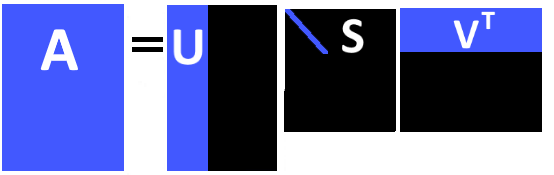
\includegraphics[width=0.7\textwidth]{figures/chapter-SVD/low_rank_decomposition_diagram}
\decoRule
\caption[Singular value decomposition illustration.]{Decomposition of input matrix $\mtrx{A}$ into diagonal matrix of singular values $\mtrx{S}$ and matrices of left and right singular vectors. Light color illustrates low-rank approximation.}
\label{fig:lowrank_svd}
\end{figure}


Compression based on a low-rank approximation matrix is a lossy compression method. To quantify the error, the Normalized root-mean-square deviation ($\mathit{NRMSD}$) is used. It is defined as

\begin{equation}
\mathit{NRMSD} = \frac{\mathit{RMSD}}{X_{max}-X_{min}}=\frac{\sqrt{\mathit{MSE}}}{X_{max}-X_{min}},
\label{eq:nrmsd-def}
\end{equation}

\noindent
where $X_{min}$ and $X_{max}$ are elements of input matrix $\mtrx{A}$ with minimum and maximum value, respectively. This error metric is able to measure and compare errors in datasets with different scales. Therefore, it is the main parameter that is used to control the quality of compression in the proposed compression algorithm.

\section{Implementation}

Results from the finite element method are scalar, vector, or tensor fields represented by discrete values calculated in nodes of the mesh or in integration points on finite elements. In order to compress data, an auxiliary matrix~$\mtrx{A}$ has to be assembled from the results. The number of rows of the matrix~$\mtrx{A}$ is equal to the number of incremental or time steps while the number of columns is equal to the number of points in which the results are stored. Such auxiliary matrix is assembled for each scalar field and for each component of the vector and tensor fields. It means, three matrices corresponding to the displacement in the $x$, $y$, and $z$ directions are assembled for the vector of displacements in three-dimensional problems.

There are two main reasons to store particular results in separate matrices. First, the size of matrices is smaller than the size of a matrix which contains all results and therefore SVD will be performed faster. Second, the magnitudes of particular fields are very different (the stress tensor components are several order of magnitude larger than the components of the displacement vector) and the data compression algorithm would suppress the fields with small magnitudes. Once the matrix $\mtrx{A}$ is assembled for each field, the compression algorithm can be applied on it. It is purely algebraic procedure and no information about geometry of the mesh is needed.

Let us assume that the matrix is not empty and it is full rank. Then it follows from the formula (\ref{eq:cr-def}) that if $r$ is equal to the rank of matrix $\mtrx{A}$, the compression ratio is always higher than one. In other words the memory consumption of stored decomposition is bigger than the size of the original matrix. To make the compression algorithm applicable, the parameter $r$ must satisfy the condition

\begin{equation}
r<\frac{m n}{m+n+1}.
\label{eq:r-ineq}
\end{equation}

\noindent
Considering the usual shape of matrix containing FEM results, this inequality is easily satisfiable even for the $r$ being close to the rank of the original matrix as in the typical case the number of nodes or integration points is much higher than the number of analysis steps and therefore $m \ll n$.


\section{Randomized SVD}

There are many algorithms with different approaches to compute singular value decompositions. One approach is based on diagonalization of the matrix which essentially yields the whole decomposition at the same time. The other approach is the use of an iterative algorithm that yields one or several singular values at a time and can be stopped after desired number of singular values and vectors has been computed. Although these algorithms have proven to work very well for relatively small matrices, they are not well suited for using with large data sets. The exact SVD of a $m \times n$ matrix has computational complexity $\mathrm{O}(\mathrm{min}(mn^2, m^2n))$ using the ``big-O'' notation. When applied on large data sets it tends to be very time-consuming. Also, the modern hardware architectures use caches to optimize reading of consecutive memory blocks. As these algorithms often need random access to the memory where the input matrix is stored, it can increase communication between different levels in memory hierarchy, which causes higher latency when accessing data. From a numerical linear algebra perspective, an additional problem resulting from increasing matrix sizes is that noise in the data, and propagation of rounding errors, become increasingly problematic.

In \cite{Woolfe2008, Candes2011, Martinsson2011}, there are described randomized methods for constructing approximate matrix factorizations which offer significant speedups over classical methods. The particular implementation of the randomized decomposition is based on the algorithm described in \cite{Halko2011}. The authors proposed an algorithm for efficient computation of low-rank approximation to a given matrix. The method uses random sampling to identify a subspace that captures most of the action of a matrix. The input matrix is compressed to this subspace, and deterministic manipulations are then used to obtain the desired low-rank factorization. For a matrix that is too large to fit in fast memory, the randomized techniques require only a constant number of passes over the data, as opposed to $\mathrm{O}(k)$ passes for classical algorithms.